


در فصول قبل نحوه‌ی محاسبه‌ی انرژی انحنا و کششی سطوح دو بعدی را مطالعه کردیم. حال فرض می‌کنیم که یک رویه‌ی دو بعدی با هندسه‌ی بسته در اختیار داریم که حجم کاهیده‌ی آن نزدیک به یک کُره است. سطح این رویه به علت اُفت و خیز ترمودینامیکی محیط دائم در حال تغییر است. در صورتی که یک لحظه زمان را متوقف کنیم، رویه‌ای خواهیم داشت که سطح آن پُر از برآمدگی و فرورفتگی در مکان‌های تصادفی است. اگر فرض کنیم اطلاعات مکانی تمام نقاط روی سطح را در اختیار داشته باشیم چطور می‌توانیم انرژی انحنا یا انرژی کشش این سطح را اندازه‌گیری کنیم؟ 

\begin{figure}[h]
\begin{center}

\includegraphics[width=\columnwidth]{\MemFluc /Pics/signal_1}
\caption{
 ریسمانی در حال افت و خیز در فضای دو بعدی. 
}
\label{fig:flucString1}
\end{center}
\end{figure}


حالا فرض کنیم که مسئله‌ی ساده‌تری را مطالعه می‌کنیم. فرض کنیم که به جای رویه، یک ریسمان در اختیار داریم که دو سر آن ثابت است و ریسمان  در یک فضای ۲ بعدی  در حال افت و خیز است. در شکل 
\ref{fig:flucString1},
چیدمان این ریسمان در زمان تصادفی‌ رسم شده‌است.
\begin{figure}[t]
\begin{center}
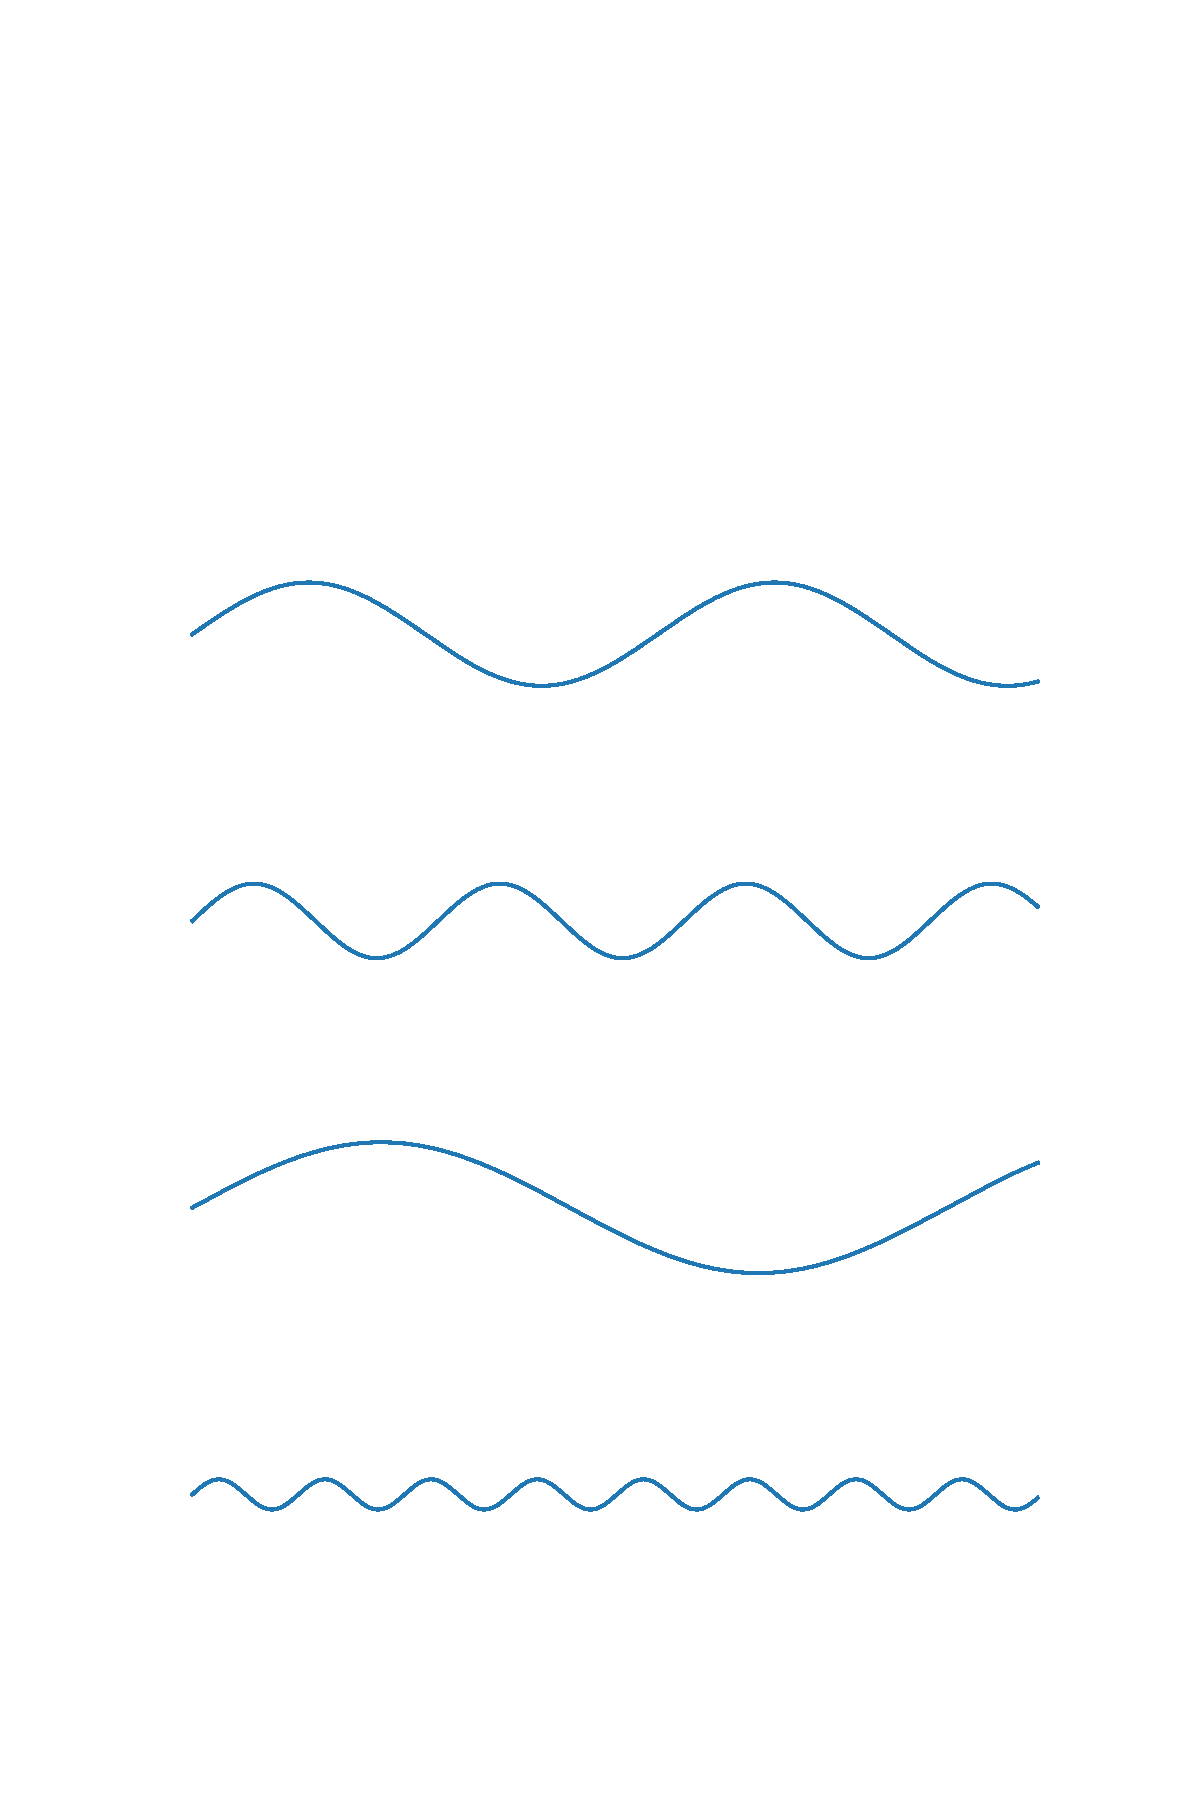
\includegraphics[width=5in]{\MemFluc /Pics/signal_2}
\caption{
مُدهای نرمال تشکیل دهنده‌ی ریسمانِ شکل
\ref{fig:flucString1}
را نشان می‌دهد. ریسمان از چهار مُد نرمال با فرکانس و شد‌ت مختلف ساخته شده‌است. 
}
\label{fig:flucString2}
\end{center}
\end{figure}
در صورتی که لازم باشد اطلاعات ساده‌ای مانند انرژی جنبشی یا انرژی پتانسیل این ریسمان محاسبه شود، با فرض اینکه اصل برهم نهی بر قرار است، کافی است که مُدهای نرمال این ریسمان را پیدا کنیم. مُدهای نرمال این ریسمان با توابع مثلثاتی تعریف می‌شوند. با محاسبه‌ی مجموع انرژی جنبشی یا پتانیسل مُدهای تشکیل دهنده‌ی این شکل می‌توانیم انرژی کلی جنبشی یا پتانسیل این ریسمان را محاسبه کنیم. در شکل
\ref{fig:flucString2}
مد‌های تشیل دهنده‌ی این ریسمان رسم شده‌است.



 
 
 
 
 
 
 
 
 
 
 